\chapter{Results}\label{chap:results}


Describe the experimental setup, the used datasets/parameters and the experimental results achieved

This chapter will present the experimental setup and execution of research questions of this thesis, datasets, libraries and execution environments used for this purspose, following the setup and execution, experimental results obtained will be described with visual aids.

\section{Experimental setup and execution}
\subsection{Datasets}
In the first stage of the execution the datasets were collected with a small window of filtering for Autosklearn since it uses 140 of the openly available datsets in there meta-learning method. Openml\cite{OpenML2013} api was used to fetch the meta data to describe each dataset. The data sets in the table \ref{tbl:datasets} were chosen by excluding the ones listed in this paper\cite{autosklearn_supplementary}

\begin{table}[]
\label{tbl:datasets}

\begin{tabular}{|l|l|l|l|l|l|}
\hline
dataset name                & instances & features & classes & task\_type     & openml\_id \\ \hline
balance-scale                   & 625       & 5        & 3       & classification & 11         \\ \hline
breast-cancer                   & 286       & 10       & 2       & classification & 13         \\ \hline
diabetes                        & 768       & 9        & 2       & classification & 37         \\ \hline
tic-tac-toe                     & 958       & 10       & 2       & classification & 50         \\ \hline
irish                           & 500       & 6        & 2       & classification & 451        \\ \hline
192\_vineyard                   & 52        & 4        & 2       & regression     & 713        \\ \hline
562\_cpu\_small                 & 8192      & 13       & 2       & regression     & 735        \\ \hline
678\_visualizing\_environmental & 111       & 4        & 2       & regression     & 736        \\ \hline
195\_auto\_price                & 159       & 16       & 2       & regression     & 745        \\ \hline
579\_fri\_c0\_250\_5            & 250       & 6        & 2       & regression     & 776        \\ \hline
225\_puma8NH                    & 8192      & 9        & 2       & regression     & 816        \\ \hline
503\_wind                       & 6574      & 15       & 2       & regression     & 847        \\ \hline
505\_tecator                    & 240       & 125      & 2       & regression     & 851        \\ \hline
542\_pollution                  & 60        & 16       & 2       & regression     & 882        \\ \hline
210\_cloud                      & 108       & 8        & 2       & regression     & 890        \\ \hline
balance-scale                   & 625       & 5        & 2       & classification & 997        \\ \hline
vowel                           & 990       & 14       & 2       & classification & 1016       \\ \hline
dna                             & 3186      & 181      & 3       & classification & 40670      \\ \hline
australian                      & 690       & 15       & 2       & classification & 40981      \\ \hline
monk1                           & 556       & 7        & 2       & classification & 333        \\ \hline
Hill\_Valley\_without\_noise    & 1212      & 101      & 2       & classification & 1479       \\ \hline
\end{tabular}
\caption{Classification and Regression Datasets}
\end{table}

\subsection{Autosklearn and TPOT execution}
Python version 3 and several python packages and a database was used to execute the experiments. The default configurations of the libraries were used except the run-time limit was set to 60 minutes. Total of 20 datasets having classification and regression tasks were executed using both the libraries sequentially. The performance of each task was recorded in the database with accuracy,f1-score and the model was saved using pickle\footnote{\url{https://docs.python.org/3/library/pickle.html}}. Due to hardware limitations Parallel execution was not possible, each library took 20 hours totalling 40 hours of execution time. The experiments produced 20 models of different algorithms and 20 scores for the respective datasets. Once the results were accumulated and storing the model files in pickle format the model were reusable without any retraining from scratch. With the reusable models, statistical significance test was conducted with the result set's of both the models. The result set was acquired by re-training the model's with 30 different splits of respective dataset which it was trained before, and resulted in 30 accuracy values for each library totalling to 60 scores. Due to refit function available in both the libraries the time taken for computing 30 repetitions was lesser than the 60 minutes.

\subsection{Developing the Web Interface}
Web interface was implemented in the same python environment as the evaluation framework which is version 3, Dash Web Analytic framework was used to build the interface. Dash provides out of the box methods for creating graphs, tables, UI elements with ease and runs under a simple web server with instant changes being reflected during developmental changes from the IDE, this feature was much help full while building the layout of the interface especially with styling and positioning of the UI-elements. Dynamic behaviour of the interface was easy to carry out from Dash core components module which provides callbacks for each UI-element in the simple python function definition. Each table or graph used in the interface was re-usable hence only the underlying data had to be updated on selection of different dataset. The layout design was inspired by one of the examples provided by Dash\footnote{\url{https://dash.plot.ly/gallery}}. 

\section{Experimental Results}

The first research question of this thesis \ref{point:R1} was to compare the performance of Autosklearn and Tpot, to this question we had collected 20 datasets containing classification and regression datasets, using the two libraries the tasks were executed with all the datasets, both the libraries produced 20 different models with each model having different combination of there parameters. Autosklearn produced a final ensemble and Tpot produced best pipeline with its parameter settings. Bayesian optimization and genetic algorithm search methodology is the main area of importance to the execution of finding optimal solutions in these libraries. The evaluation criteria being the balanced accuracy and f1-score for classification problems and root mean squared error rate for regression problems along with run time, the following result sets will explain which Automatic Machine learning library performed better not only in terms of  evaluation measures also with statistical significance test.

\subsection{Classification tasks}
\label{classficationtasks}
In the table \ref{tbl:classification_tasks} from a general inspection we can  observe that model performance across the datasets are almost similar except for few models, autosklearn and tpot consecutively produced similar results on each task, we should note that each of the models are different from one another and they also have different hyperparameter configuration. The dataset monk1 has a score of 100\% through out all the measures from both the libraries, this could indicate that there might be validation with training set itself, if that is the case it should have been reproduced along other tasks as well or the dataset's distribution favours the algorithm. Autosklearn has models with less than 80\% accuracy in 3 of the tasks where as  tpot has only 2 models below 80\% this is not a huge margin difference when compared to other 2 measures, when we compute the mean of each scores we can say that the performance difference is not significant, autosklearn scores are predicted from an ensemble of models were has tpot is a single best pipeline with just one algorithm. The essential part of an ensemble is to average out the predictions from the overall predictions made this should provide a significant advantage for autosklearn but still against a single model the performance is very similar, what we can notice here is that the ensemble of models or just the single pipeline model would perform better under optimal hyperparameter configuration.By taking a general average performance across datasets tpot performs better than autosklearn in accuracy and balanced-accuracy only by a 1\% margin.

\subsection{Regression tasks}
In the table \ref{tbl:regression_tasks} describes the performance in regression tasks for both the libraries, here we can see that for the task vineyard there is a negative score which can be for root mean squared error, if we examine the reason for such a low score is due to the no of instances and features available in the dataset, there are other two datasets in which both the libraries performed very poorly. The poor performance could be from the models which are not able to obtain much information about the data and squared error gives out a huge difference, also the datasets having very few instances less than 1000, both autosklearn and tpot are unable to perform empirically. Since there is not enough data points to accumulate information the models fail to recognize changes. Overall performance across the tasks
from both the libraries is similar and only a thin margin of score difference can be seen.

\subsection{Algorithm preference and performance}
Fig \ref{fig:algorithm} gives us an estimate in percentage of how many times the estimators has been selected to build a model under autosklearn and tpot for the dataset tic-tac-toe, for autosklearn its been clearly seen that adaboost and gradient boosting which are ensemble methods are selected in majority of the times, this might be due to the final outcome being an ensemble methods handling the properties of ensemble can be a better estimator. When compared across tpot gradient boosting is the dominant estimator chosen. RandomforestClassifier and extratreesClassifier are in top 5 slot of being selected to build a pipeline in tpot since both the algorithms are better at handling when stacked with other features estimators. Fig \ref{fig:performance} explains the performance of both the libraries across different metrics for a given dataset, we can observe except for few tasks the performance is near to overlapping. Some of the tasks gained negative rmse scores while in classification below 20\% accuracy can be seen, coming to the runtime of the toolkits autosklearn managed to stay within seconds of the end minute boundary where as tpot took a 30 to 60 secs extra time to stop its execution. As explained above in section \ref{classficationtasks} why the scores are low the data at hand is very important for any algorithm to get trained efficiently.



\begin{table}[]
\centering
\begin{tabular}{|l|l|l|l|l|l|l|}
\hline
dataset\_name                & \multicolumn{2}{c|}{\begin{tabular}[c]{@{}c@{}}Autosklearn - Tpot\\  F1-score\end{tabular}} & \multicolumn{2}{l|}{\begin{tabular}[c]{@{}l@{}}Autosklearn - Tpot\\        Accuracy\end{tabular}} & \multicolumn{2}{l|}{\begin{tabular}[c]{@{}l@{}}Autosklearn - Tpot \\   balance-accuracy\end{tabular}} \\ \hline
breast-cancer                & 0.694                                        & 0.708                                        & 0.694                                           & 0.666                                           & 0.672                                             & 0.692                                             \\ \hline
diabetes                     & 0.734                                        & 0.689                                        & 0.744                                           & 0.718                                           & 0.736                                             & 0.685                                             \\ \hline
dna                          & 0.959                                        & 0.687                                        & 0.959                                           & 0.959                                           & 0.961                                             & 0.961                                             \\ \hline
monk1                        & 1.0                                          & 1.0                                          & 1.0                                             & 1.0                                             & 1.0                                               & 1.0                                               \\ \hline
tic-tac-toe                  & 1.0                                          & 0.991                                        & 1.0                                             & 0.995                                           & 1.0                                               & 0.988                                             \\ \hline
australian                   & 0.878                                        & 0.849                                        & 0.878                                           & 0.849                                           & 0.880                                             & 0.850                                             \\ \hline
balance-scale                & 0.987                                        & 1.0                                          & 0.987                                           & 1.0                                             & 0.969                                             & 1.0                                               \\ \hline
Hill\_Valley\_without\_noise & 0.693                                        & 1.0                                          & 0.693                                           & 1.0                                             & 0.697                                             & 1.0                                               \\ \hline
vowel                        & 0.991                                        & 0.983                                        & 0.991                                           & 0.983                                           & 0.992                                             & 0.984                                             \\ \hline
irish                        & 1.0                                          & 1.0                                          & 1.0                                             & 1.0                                             & 1.0                                               & 1.0                                               \\ \hline
\end{tabular}
\caption{Classification tasks}
\label{tbl:classification_tasks}
\end{table}


\begin{table}[]
\centering
\begin{tabular}{|l|l|l|}
\hline
dataset name                    & \multicolumn{1}{c|}{Autosklearn rmse} & Tpot rmse \\ \hline
503\_wind                       & 0.777                                 & 0.790     \\ \hline
225\_puma8NH                    & 0.670                                 & 0.680     \\ \hline
562\_cpu\_small                 & 0.980                                 & 0.979     \\ \hline
195\_auto\_price                & 0.888                                 & 0.837     \\ \hline
505\_tecator                    & 0.987                                 & 0.997     \\ \hline
192\_vineyard                   & 0.0153                                & -0.334    \\ \hline
579\_fri\_c0\_250\_5            & 0.950                                 & 0.944     \\ \hline
678\_visualizing\_environmental & 0.363                                 & 0.149     \\ \hline
542\_pollution                  & 0.317                                 & 0.022     \\ \hline
210\_cloud                      & 0.681                                 & 0.710     \\ \hline
\end{tabular}
\caption{Regression tasks}
\label{tbl:regression_tasks}
\end{table}

\begin{figure}[!h]
    	\centering
    	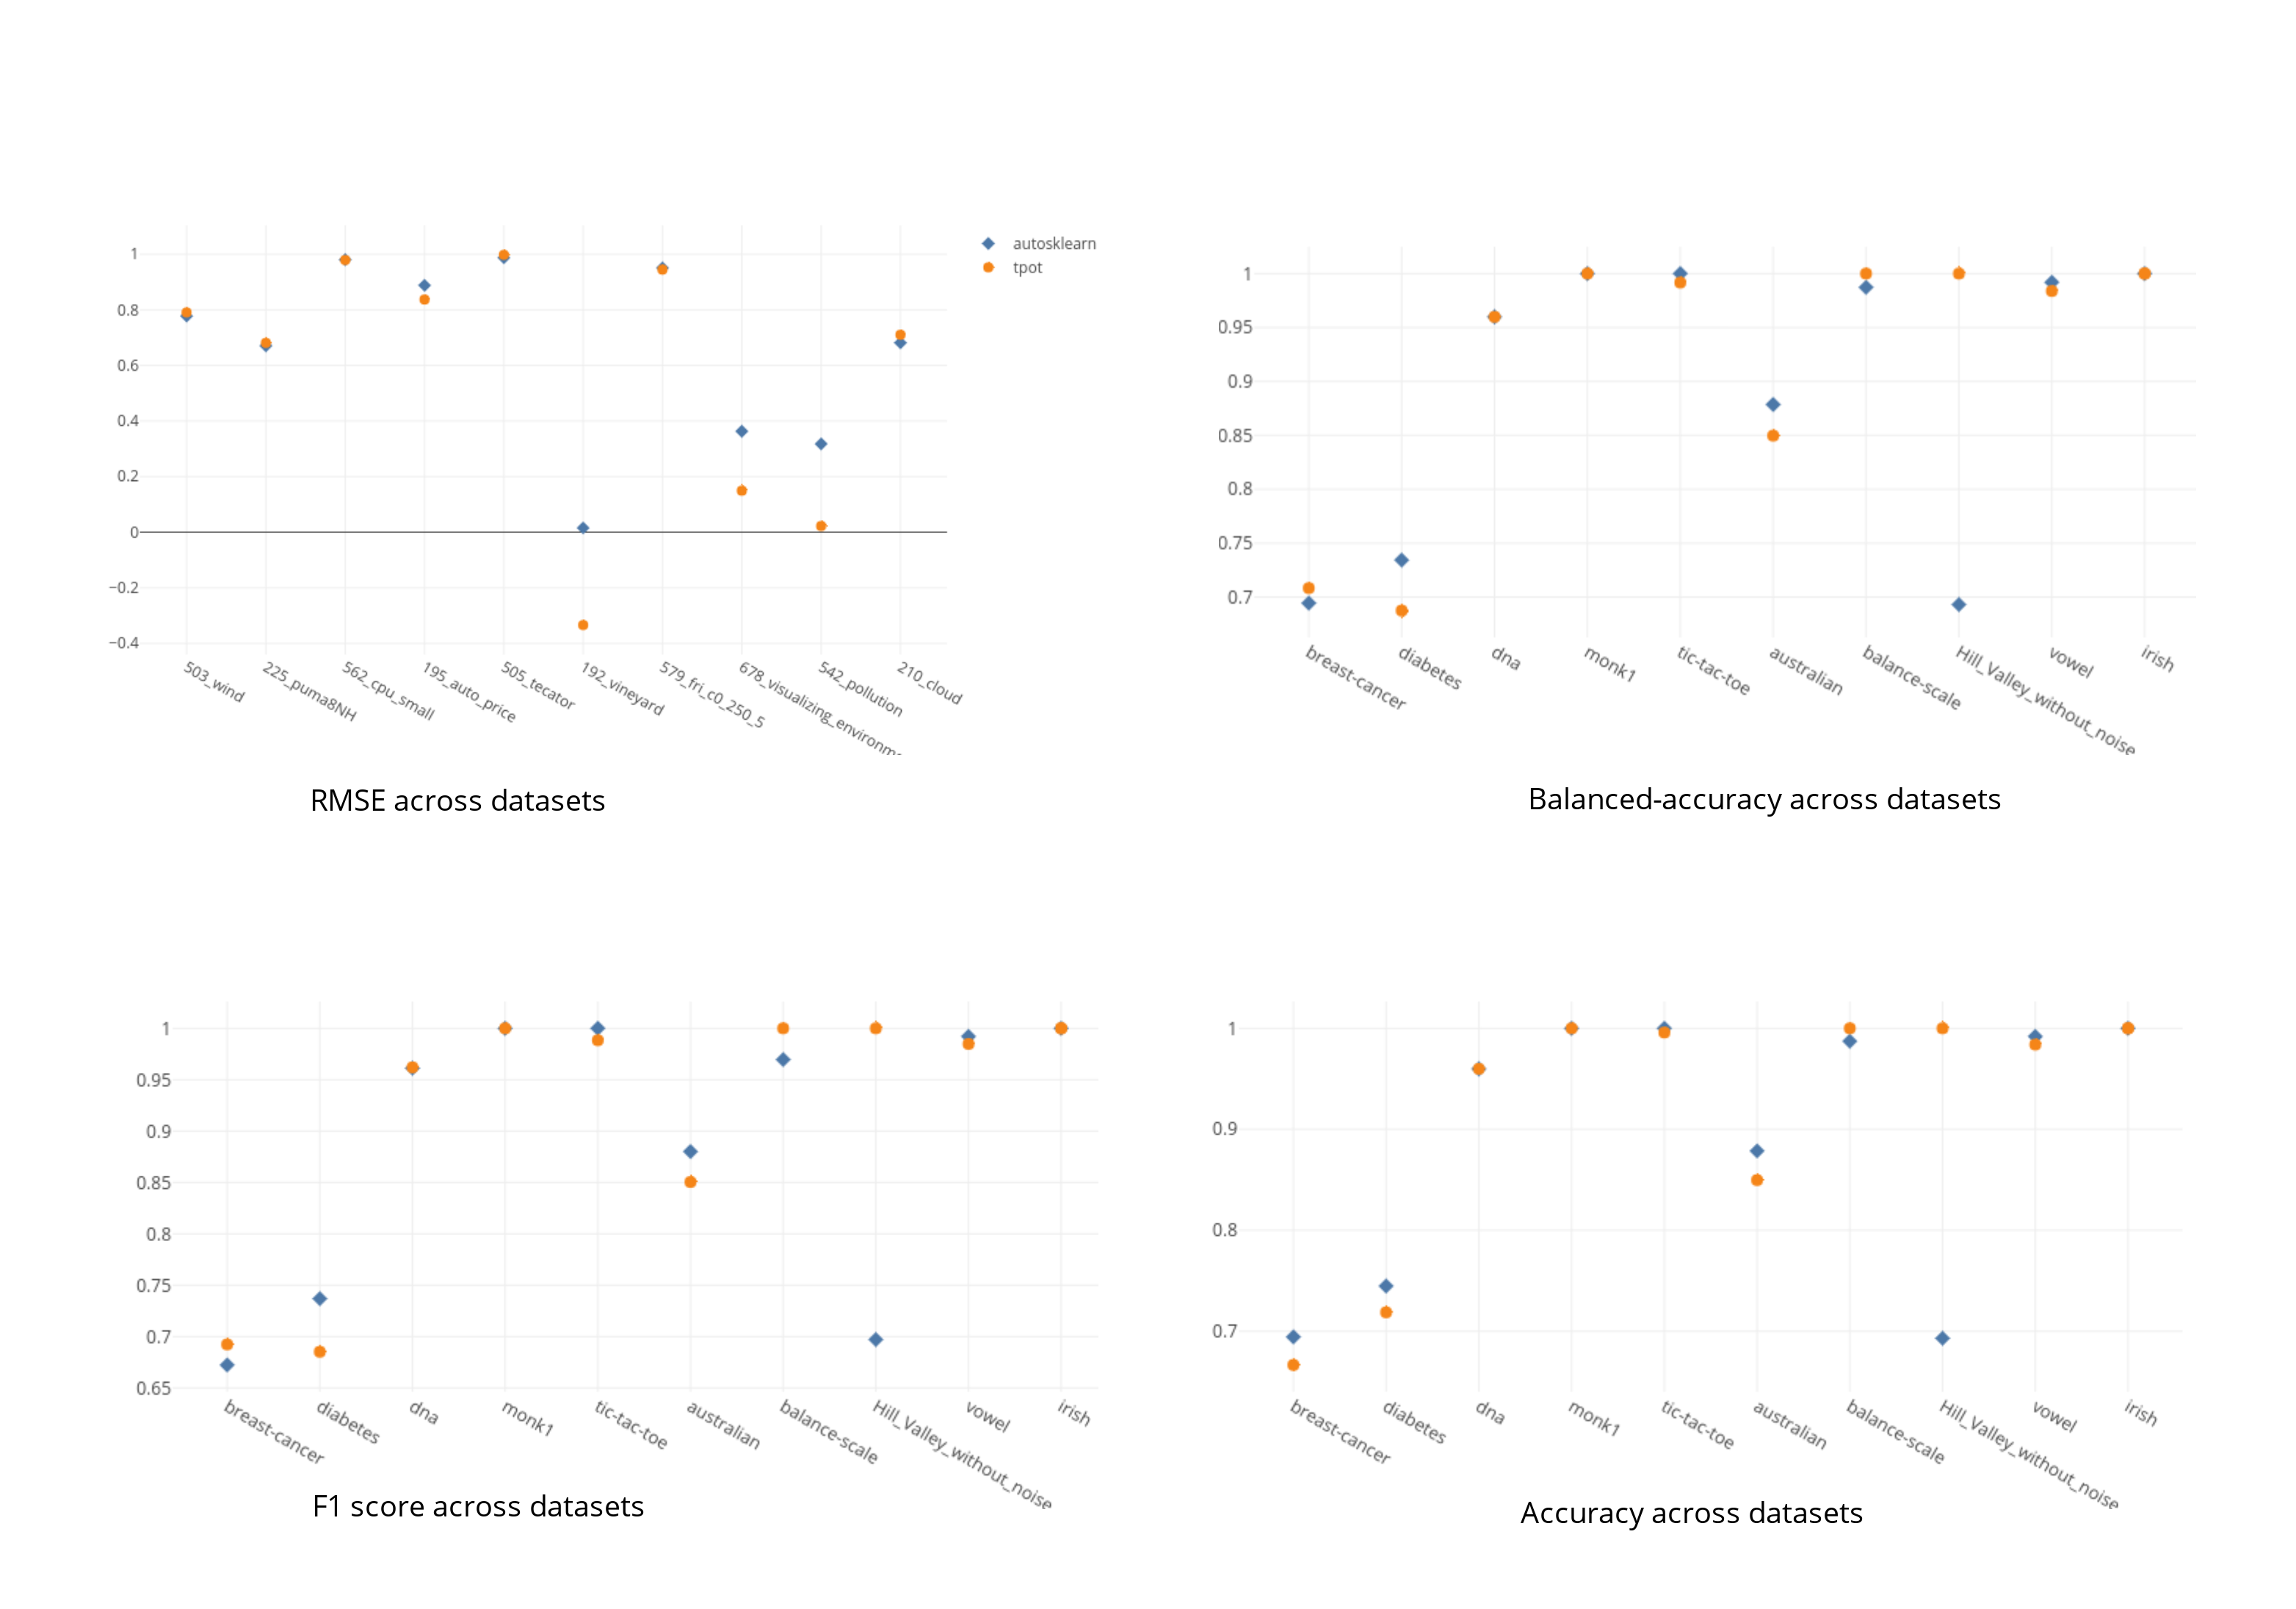
\includegraphics[width=0.9\linewidth]{thesis_template/images/performanceplot.png}
    	\caption{Performance plot across metrics}
    	\label{fig:performance}
        \end{figure}
        

\begin{figure}[!h]
    	\centering
    	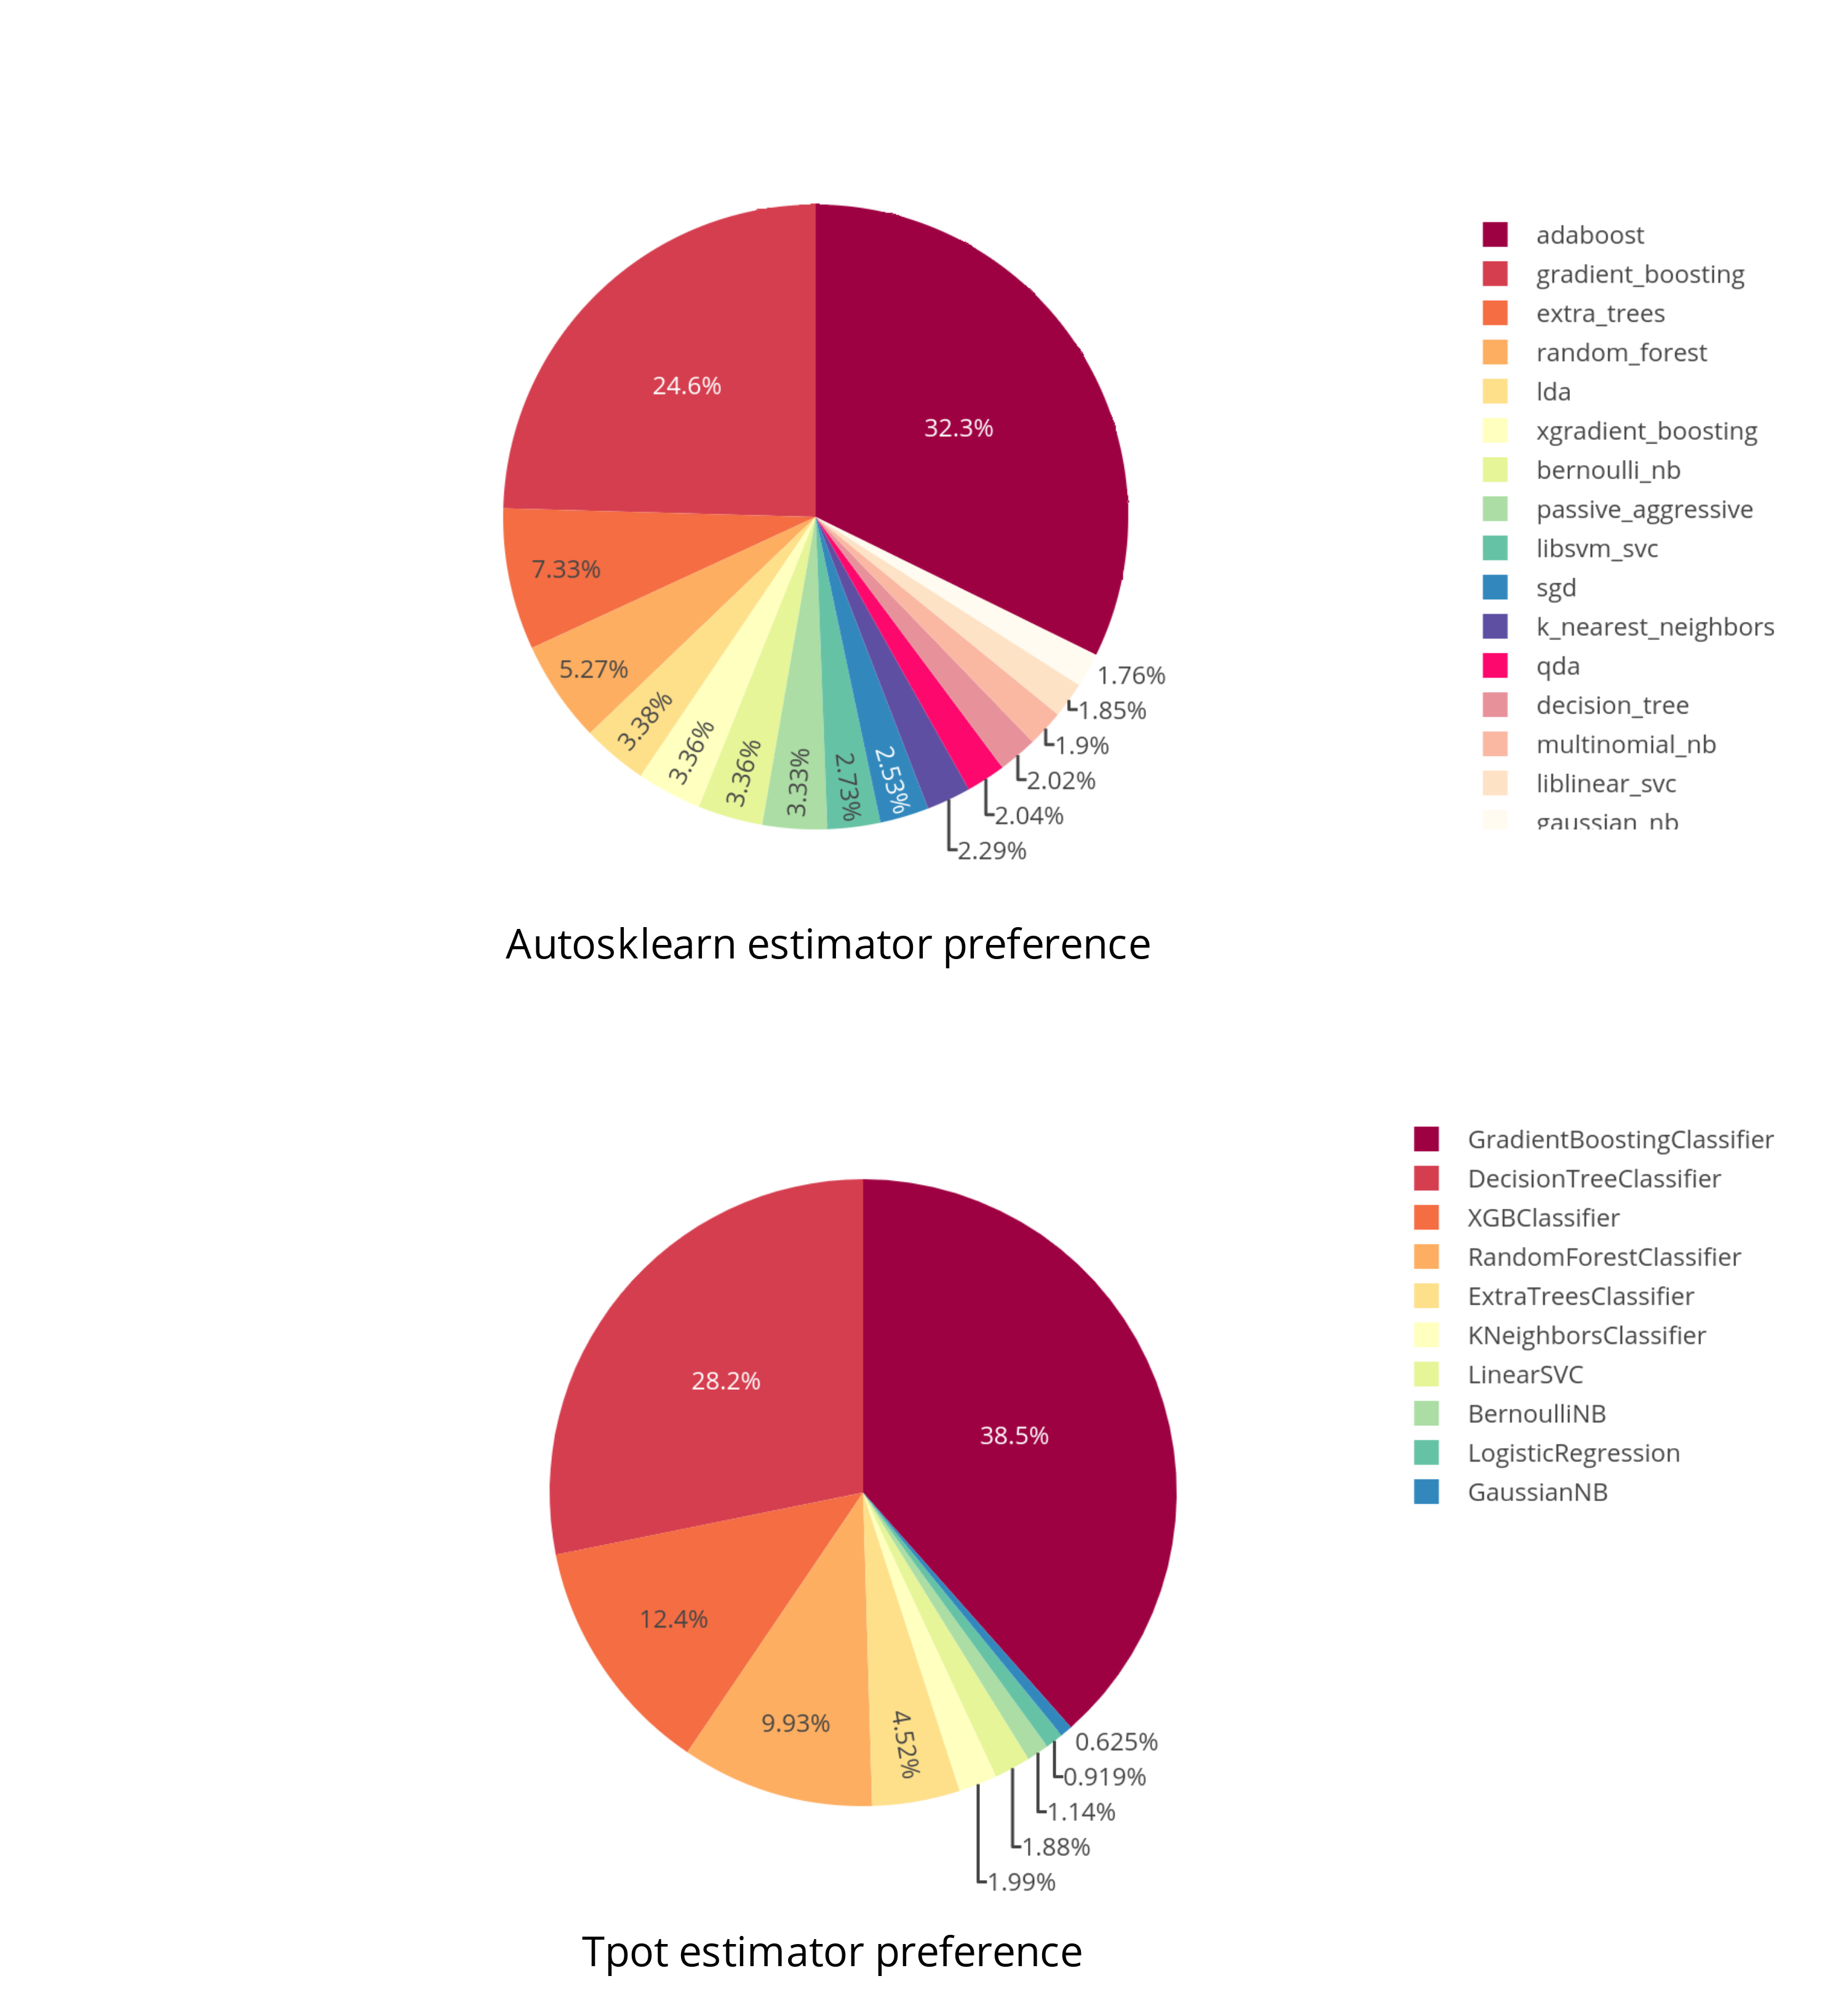
\includegraphics[width=0.8\linewidth]{thesis_template/images/pieplotBoth.png}
    	\caption{Autosklearn and tpot estimators preference on tic-tac-toe}
    	\label{fig:algorithm}
        \end{figure}



\subsection{Statistical significance}

Statistical significance is an essential tool to asses the performance when comparing two different algorithms, the significance comes into picture were we need to effectively and quantitatively examine the difference between the two methods. The methods are different in the terms of there methodolgy employed, but when the goal of the methods is to maximize a function with the given costs the obtained outcomes would be similar. The outcome can be similar but how the methods reach that outcome is different in there own ideology and mechanism. When the result is achieved by the methods based on a certain criteria we only asses the methods based on the sole criteria and overlook on how the methods achieved the result, to quantify these methods the second research question in this thesis R2 \ref{point:R2} is to conduct a statistical significance test among the top performing models from both the libraries. A simple hypothesis stating "The samples of scores are correlated" is the assumption made, since the evaluation experiments are done only once a certain set of repeated samples would give us a distribution of results to examine, for this 20 repeated model training was done on 20 different splits of data finally 20 scores were obtained from the task. Table \ref{tbl:significance} has entries of classification and regression tasks which performed above 90\% from both the libraries. spearmanr\footnote{\url{https://docs.scipy.org/doc/scipy-0.14.0/reference/generated/scipy.stats.spearmanr.html}} statistical test was used to compute the p-values of each model, the accumulated scores are not shown in the table only the p-value which is obtained from the test is displayed to describe the tasks. Out of 12 models 8 models between tpot and autosklearn values are correlated on 20 different train test splits, a alpha value of 0.05 was selected as the standard measure for p-value. The 8 models which are correlated describes the behaviour as similar for both the libraries, from comparing the performance scores in the tables \ref{tbl:classification_tasks}, \ref{tbl:regression_tasks} and as we saw the thin margin difference in there scores, statistical significance test shows that the two libraries perform similarly and this could be due to the algorithm and hyperparameter optimization from both the libraries which essentially tackled the search space on a similar scale. For the samples which are uncorrelated indicates the algorithm configuration obtained is different with other models.

\begin{table}[]
\centering
\begin{tabular}{|l|l|l|}
\hline
dataset\_name        & p\_value               & significance       \\ \hline
562\_cpu\_small      & 0.00015231             & Samples are correlated   \\ \hline
505\_tecator         & 0.5352473458918693     & Samples are uncorrelated \\ \hline
balance-scale        & 0.10498579026636898    & Samples are uncorrelated \\ \hline
vowel                & 0.0052                 & Samples are correlated   \\ \hline
195\_auto\_price     & 0.1316                 & Samples are uncorrelated \\ \hline
225\_puma8NH         & 0.000000002            & Samples are correlated   \\ \hline
503\_wind            & 0.000000035            & Samples are correlated   \\ \hline
579\_fri\_c0\_250\_5 & 0.1426                 & Samples are uncorrelated \\ \hline
australian           & 0.0003                 & Samples are correlated   \\ \hline
breast-cancer        & 0.0012                 & Samples are correlated   \\ \hline
diabetes             & 0.0001                 & Samples are correlated   \\ \hline
dna                  & 0.0000511              & Samples are correlated   \\ \hline
\end{tabular}
\caption{Statistical Significance between tpot and autosklearn}
\label{tbl:significance}
\end{table}

\begin{figure}[!h]
    	\centering
    	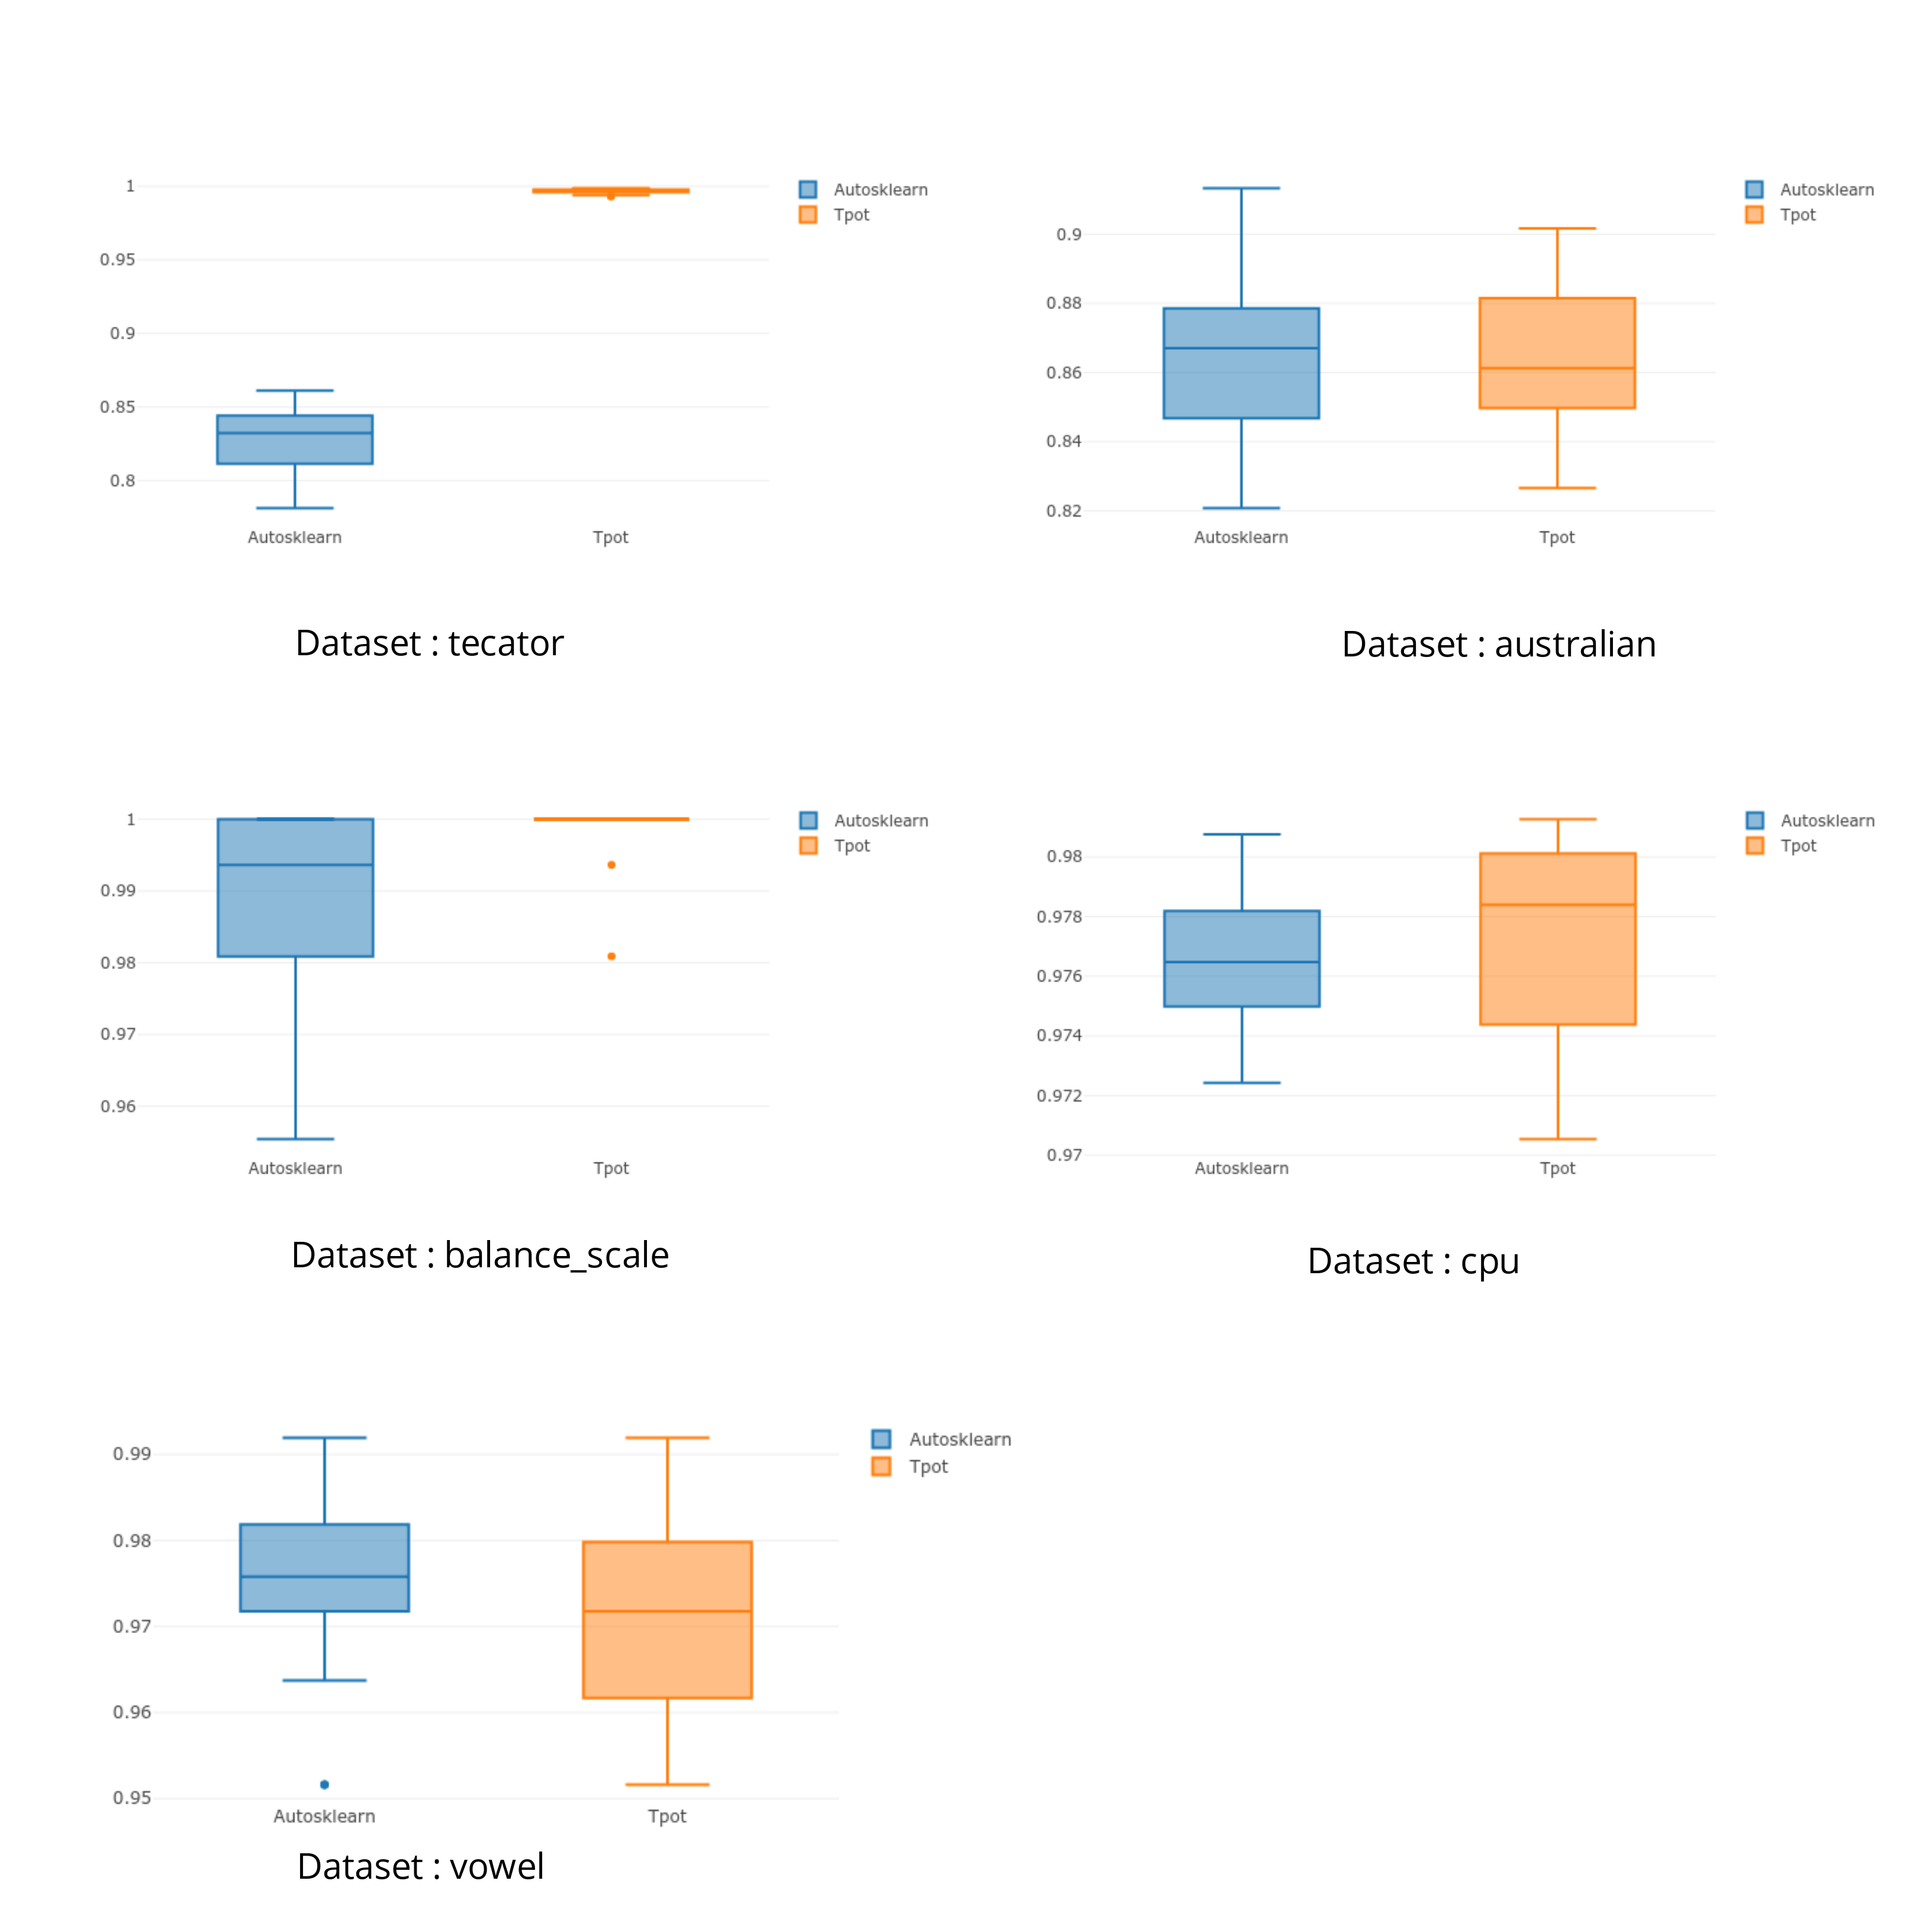
\includegraphics[width=0.84\linewidth]{thesis_template/images/significance.png}
    	\caption{Statistical significance across tasks}
    	\label{fig:significance}
        \end{figure}
        
Fig \ref{fig:significance} has the box plots of some of the models chosen from the list in the table \ref{tbl:significance} here we can see both tpot and autosklearn how they are being uncorrelated on a particular task, for example the tecator dataset there is huge difference in the distribution of scores and for balance-scale there are outliers in the distribution. Below are some of the algorithms with there hypereparameters chosen by the respective library for the particular task. The models shown below in the section \ref{auto:hyp} , \ref{tpot:hyp} are specifically selected to examine the different parameters which are responsible for the models performance.

\subsection{Autosklearn algorithms with hyperparmeters}
\label{auto:hyp}
\begin{itemize}
\item 
Dataset CPU : Algorithm : \textbf{RandomForest}

\begin{spverbatim}
{'bootstrap': True, 'criterion': 'mse', 'max_depth': None, 'max_features': 1.0, 'max_leaf_nodes': None, 'min_impurity_decrease': 0.0, 
'min_impurity_split': None, 'min_samples_leaf': 1, 'min_samples_split': 2, 'min_weight_fraction_leaf': 0.0, 'n_estimators': 100, 'n_jobs': 1, 
'oob_score': False, 
'verbose': 0, 'warm_start': True}
\end{spverbatim}

\item
Dataset Balance scale : Algorithm : \textbf{ LibSVM SVC}
\begin{spverbatim}
{'C': 10506.07883709228, 'cache_size': 200, 'class_weight': None, 'coef0': -0.9194756791062237, 'decision_function_shape': 'ovr', 'degree': 3, 'gamma': 0.012743229122052542, 'kernel': 'sigmoid', 'max_iter': -1.0, 'probability': False, 'random_state': <mtrand.RandomState object at 0x7fab2fdad9d8>, 'shrinking': False, 'tol': 0.037066558075681134, 'verbose': False}
\end{spverbatim}

\item
Dataset Australian : Algorithm : \textbf{LDA}
\begin{spverbatim}
{'n_components': 231, 'priors': None, 'shrinkage': 'auto', 'solver': 'lsqr', 'store_covariance': False, 'tol': 0.0001272335874479544}
\end{spverbatim}

\end{itemize}

\subsection{Tpot algorithms with hyperparmeters}
\label{tpot:hyp}
\begin{itemize}
\item 
Dataset CPU : Algorithm : \textbf{XGBRegressor}
\begin{spverbatim}
{'base_score': 0.5, 'booster': 'gbtree', 'colsample_bylevel': 1, 'colsample_bytree': 1, 'gamma': 0, 'learning_rate': 0.1, 
'max_delta_step': 0, 'max_depth': 9, 'min_child_weight': 20, 'missing': nan, 
'n_estimators': 100, 'n_jobs': 1, 'nthread': 1, 'objective': 'reg:linear', 
'random_state': 0, 'reg_alpha': 0, 'reg_lambda': 1, 'scale_pos_weight': 1, 
'seed': None, 'silent': True, 'subsample': 1.0}
\end{spverbatim}

\item

Dataset Balance scale : Algorithm : \textbf{LogisticRegression}
\begin{spverbatim}
{'C': 10.0, 'class_weight': None, 'dual': False,'fit_intercept': True,
'intercept_scaling': 1, 'max_iter': 100, 'multi_class': 'ovr', 'n_jobs': 1,
'penalty': 'l2', 'random_state': None, 'solver': 'liblinear', 'tol': 0.0001, 
'verbose': 0, 'warm_start': False}
\end{spverbatim}

\item

Dataset Australian : Algorithm : \textbf{LogisticRegression}
\begin{spverbatim}
{'C': 20.0, 'class_weight': None, 'dual': False, 
'fit_intercept': True,'intercept_scaling': 1, 'max_iter': 100,
'multi_class': 'ovr', 'n_jobs': 1,'penalty': 'l1', 'random_state': None, 'solver': 'liblinear', 'tol': 0.0001,'verbose': 0, 'warm_start': False}
\end{spverbatim}

\end{itemize}

\subsection{Web Interface}

\begin{figure}[!h]
    	\centering
    	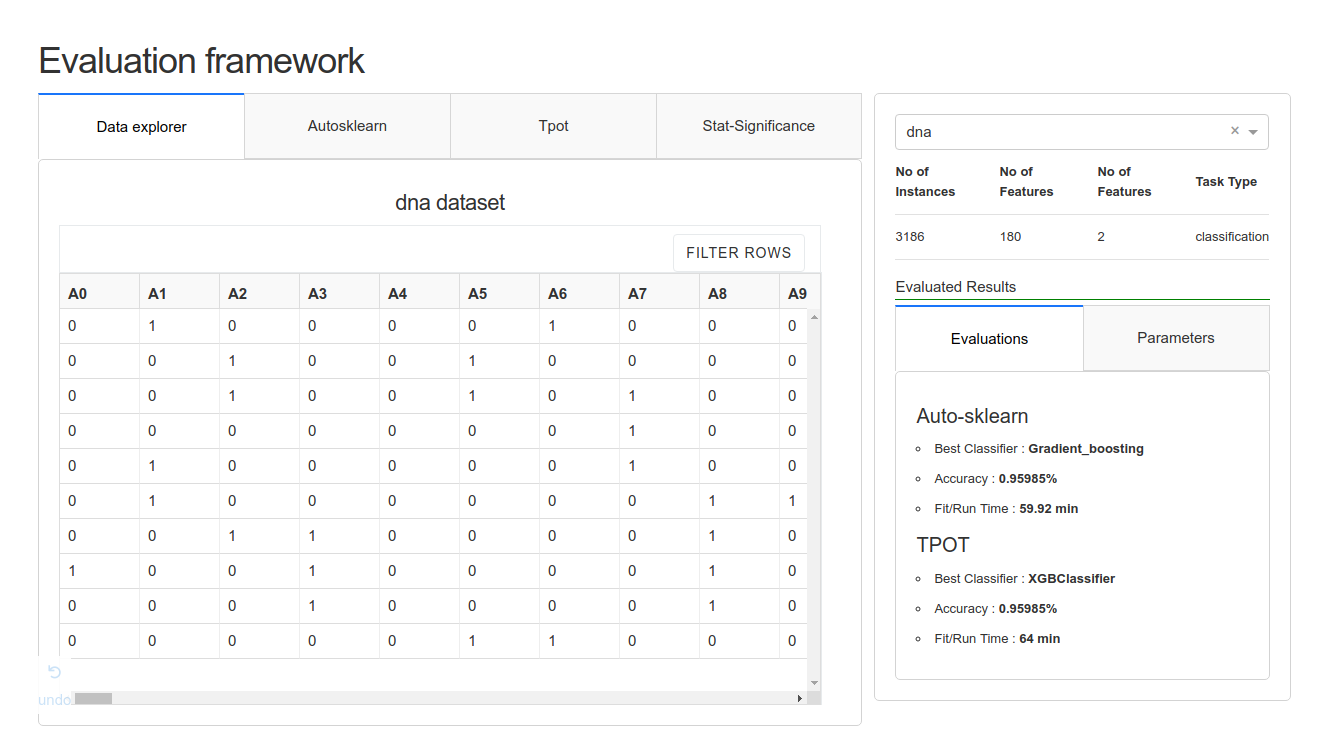
\includegraphics[width=1\linewidth]{thesis_template/images/webinterface.png}
    	\caption{Web interface}
    	\label{fig:webinterface}
        \end{figure}

The implementation of web interface was done in python environment using Dash framework, the layout of the interface was inspired by one of the apps in the dash gallery. The tabbed layout provides quick navigation between contexts and faster execution when compared to loading a entire different page, in order to keep the control sequence as simple as possible there is only one action point in the interface that is selection of dataset at the top right using a dropdown.
Maintaining a flow of observations was the key base for developing the interface, in machine learning workflow were a dataset at first is examined before selecting the algorithms for building a model, here in the web interface we first analyze the dataset which is selected using the dropdown and the table on the left hand side of the page. The table displays 10 rows which is sufficient to get a general idea about the dataset. Below the select dataset dropdown we can get the details of the dataset on its properties as No of instances,features,classes and type of task for the particular datset.

\begin{figure}[!h]
    	\centering
    	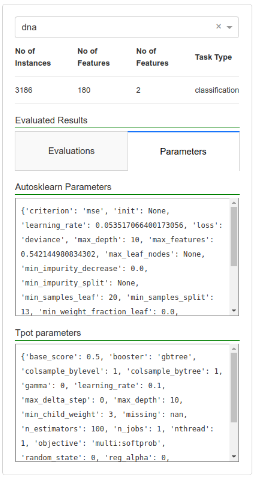
\includegraphics[width=0.4\linewidth]{thesis_template/images/parametersInterface.png}
    	\caption{Parameter tab}
    	\label{fig:parameters}
        \end{figure}


The first part of the interface is the action part were the user selects a dataset, the second part of the interface is to fetch the corresponding dataset details from the database. At any given point of time the whole page and tabs of the interface contains details only about the selected dataset except for the statistical significance tab which contains data on best models obtained from both the libraries, this is due to keeping the interface distraction free and only focus on that particular problem selected. Once selection is done the best models obtained from both the libraries are displayed under the select dropdown button in fig \ref{fig:webinterface}.
The section named Evaluated results has two tabs one is for description of the models and the second parameter tab to display the hyperparameters of that particular model. The section displays each model's brief information such as algorithm,performance score and runtime as well as the hyperparameters in the parameter tab as seen in fig \ref{fig:parameters} 

The Initial model details displayed is the best estimator found by both libraries, for autosklearn it is the first model in the whole final ensemble and for tpot it is the best pipeline obtained and the corresponding hyperparameters as well. The four bigger tabs on the left hand side of the page are namely, Data explorer, Autosklearn, Tpot and statistical significance.
The data explorer tab as shown in the fig \ref{fig:webinterface} displays the rows of the dataset to examine at first, the next tab in the line Autosklearn lists the rest of the models details found in the final ensemble excluding the one which is displayed on selection of the dataset. Same ideology for tpot tab as well were the individual pipelines examined  by tpot library to find the best models at last.At last is the statistical significance tab were its not in connection with selection of dataset or any other actions performed. The tab lists the models whose performance is above 90\%  and some models with very low accuracy in the overall 20 tasks taken up by autosklearn and tpot. Fig \ref{fig:signi} is the section were outcome is represented with boxplots in fig \ref{fig:signiplots} each outcome is a collapsible container which encloses box plots and parameters of that particular model and dataset. Below the box plot, the hyperparameters for both autosklearn and tpot are listed to grab information about the task without any navigation.

The data displayed in the interface is already stored in the format which would aid easier integration for display formatting. JSON\footnote{\url{https://www.json.org/}} data structure is used to save and retrieve data, the evalution framework saves data in json format to aid the web interface with minimal processing of data while displaying. The whole interface is a single page application which can also be packaged and since its written in python, execution of backend scripts can be done within the callbacks of the interface itself if required, although its not recommended to perform intensive tasks at the user interface side. The interface also does not reload at every selection of dataset, it uses AJAX\footnote{\url{https://en.wikipedia.org/wiki/Ajax_(programming)}} protocol to load data and display it without reloading the whole page.The interface can be used to gain information on different models and its parameters generated by autosklearn and tpot. Apart from being built specifically to evaluate  the two libraries, the interface can give us information on variety of hyperparameters and the combinations tested, this is from the execution of Autosklearn and Tpot.

\begin{figure}[!h]
    	\centering
    	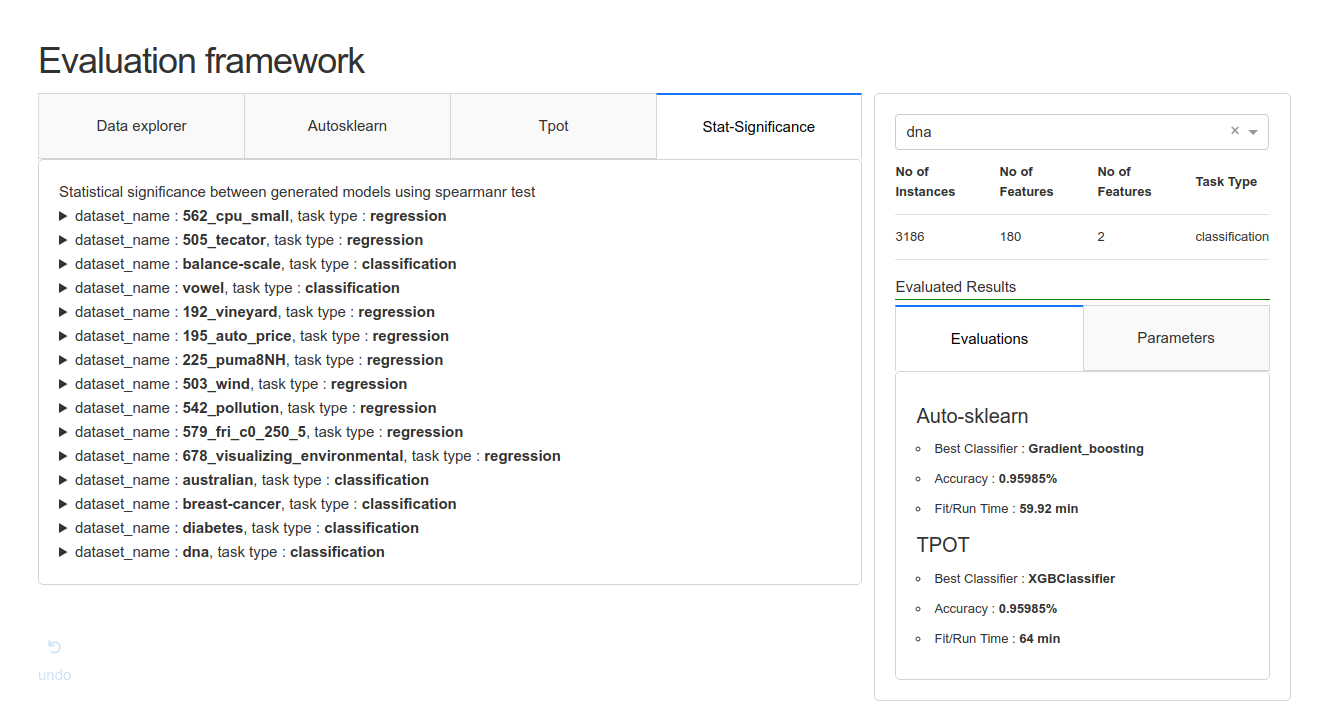
\includegraphics[width=0.9\linewidth]{thesis_template/images/statistical.png}
    	\caption{Statistical significance tab}
    	\label{fig:signi}
        \end{figure}
        

\begin{figure}[!h]
    	\centering
    	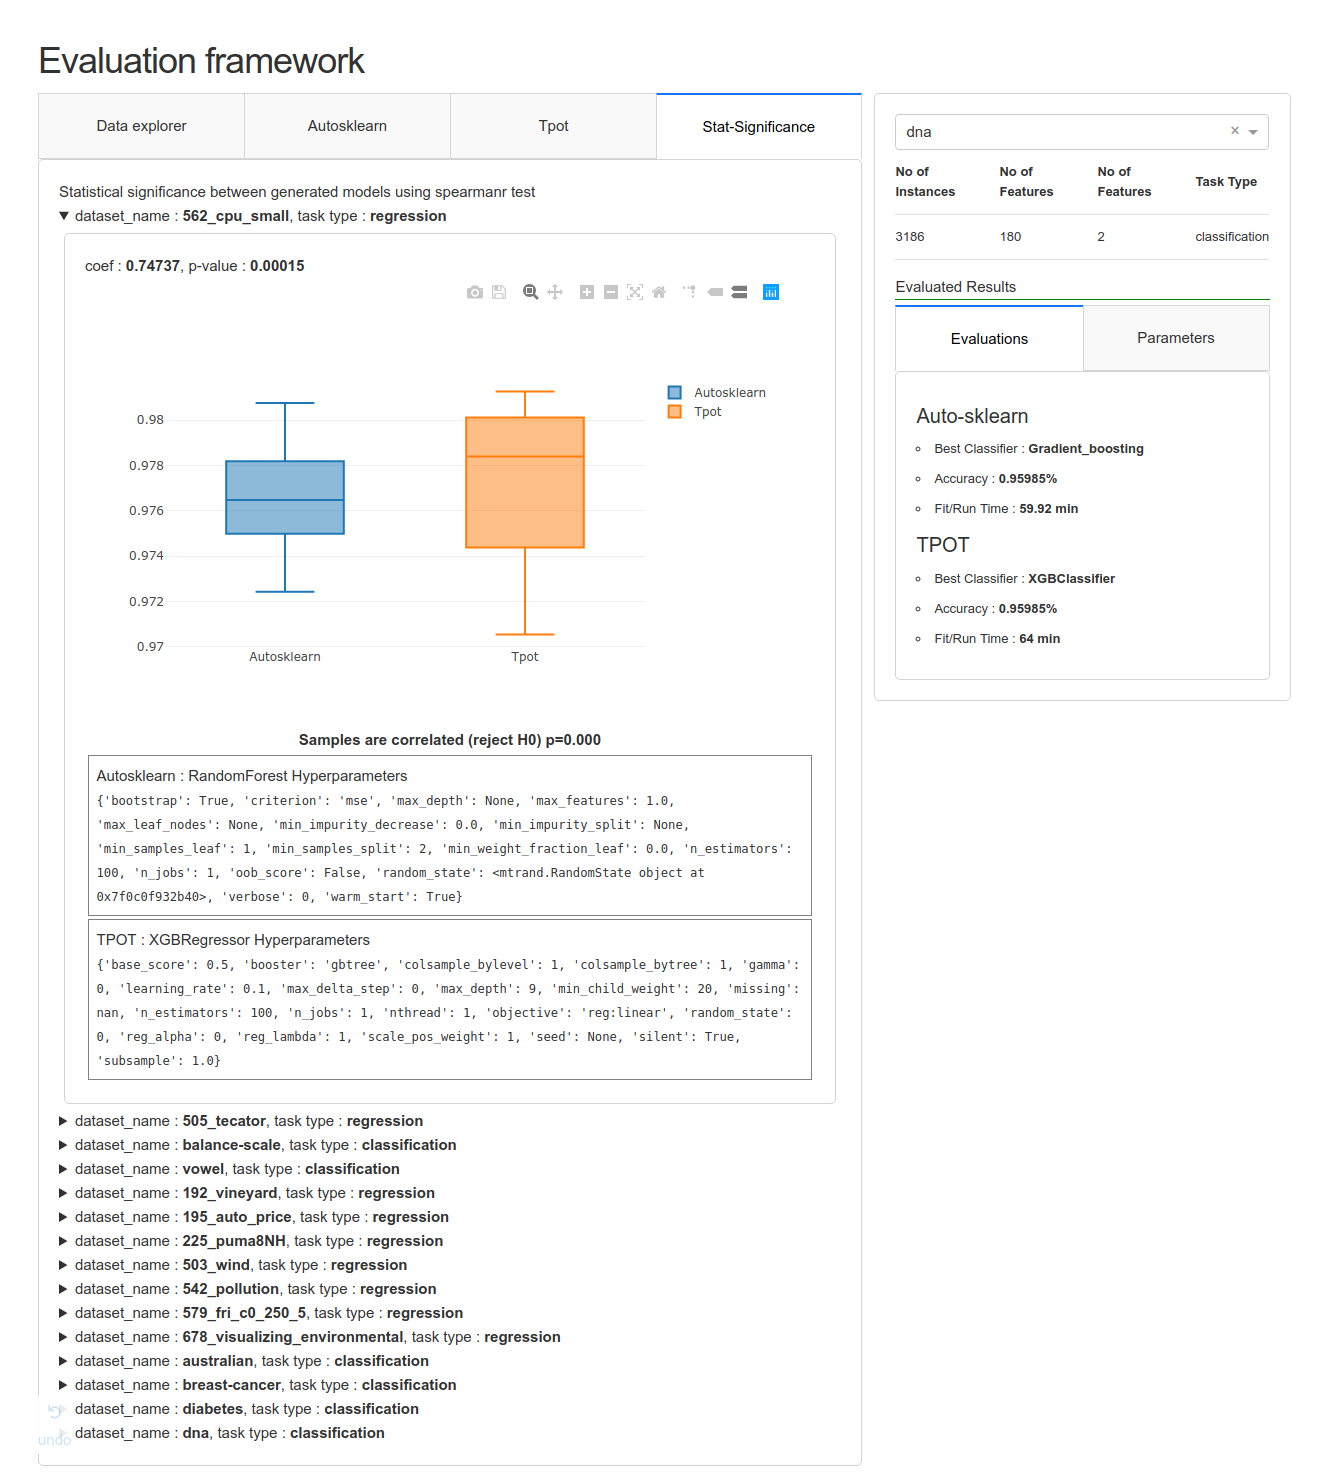
\includegraphics[width=0.9\linewidth]{thesis_template/images/statwithgraph.png}
    	\caption{Statistical significance tab with plots}
    	\label{fig:signiplots}
        \end{figure}